\chapter{Theory of RTOS\label{part:rtos-theory}}

In order to understand how a real-time operating system (RTOS) works compared to a general purpose operating system (OS),
    it is essential to define some recurrent characteristics we would expect to find in a real-time architecture.
\\
This chapter is non exhaustive and we could debate about the importance of some characteristics compared to some others.
We decided to chose those characteristics because they are commonly used in the literature
    and we think that they will provide a good glance at what we can expect from an RTOS.

%useful or not?
The first part of this thesis is the result of an effort from ours to summarize the knowledge we collected during our researches.
We spent countless hours collecting data, reading papers, documentation and technical datasheets from vendors, researchers and developers.
We also spent time contacting qualified people to review, read and advise us on very specific topics.


\section{System architecture}

Operating systems for embedded devices started appearing in the 00's.
Since then design choices have evolved with the technology, researches and trends.
\\
In this section, we will explain the different kernel architectures commonly found in RTOS and their impact on the operating system.

\subsection{Kernel}
The kernel is the center piece of an operating system.
The role of the kernel is to manage every critical function of an operating system.
The kernel could technically run by itself but it wouldn not be very practical.
An operating system is built around its kernel and in the case of an RTOS, kernel design is critical for ensuring strict deadlines.
The tasks a kernel usually manages consist in:
\begin{itemize}
    \item Memory management
    \item Process and CPU scheduler
    \item Device drivers
    \item System calls
\end{itemize}


\subsection{User space and kernel space}
Almost every operating system makes the distinction between user space and kernel space.
The memory allowed to the operating system is divided into two distinct segments.
The goal is to provide memory and hardware protection against malicious or faulty behaviors.

The first one, the kernel space, is dedicated to operations the most related to the hardware.
It is reserved for the most sensitive operations of the operating system.
Due to its central position in the operating system, any bug in the kernel can lead to system failure.
In order for an user process to use the hardware, it must ask permission to the kernel through an API so that the kernel performs the operation for the process.

The second one, the user space is dedicated to all the code running outside of the kernel space such as applications, programs and libraries.
Each user-space process has its own memory space and cannot access the memory of another process (unless they use shared memory).

\subsection{CPU modes}
%https://minnie.tuhs.org/CompArch/Lectures/week07.html
%https://blog.codinghorror.com/understanding-user-and-kernel-mode/
\paragraph{}
CPU run on different operating modes (also called states or levels).
In kernel mode (also called privilege mode or unrestricted mode), the CPU may perform any operation without restriction.
In user mode, direct access to hardware is prohibited.

Those modes prevent the application software from accessing the hardware directly.
Applications are restricted to their address space 
    and should use the operating system's abstract services in order to perform operations on the hardware.

\subsection{Interprocess communication}
%https://www.geeksforgeeks.org/interprocess-communication-methods/
Interprocess communication (IPC) designates the mechanisms used to share data between processes in an operating system.
Those mechanisms can differ from OS to OS but are generally the same.
We can notably cite:
\begin{itemize}
    \item Pipes
    \item Names pipes
    \item Message queuing
    \item Semaphores
    \item Shared memory
    \item Sockets
\end{itemize}

\subsection{Interrupt}
An interrupt is a signal emitted by hardware or software to the CPU signaling an event.
When an interrupt happens, the state of the current program is saved 
    and the routine related to the interrupt is executed.

The origin of an interrupt can be of all sort, 
    from changing running thread in a single core processor to pressing a key in a keyboard.

\subsection{Kernel architecture}

\subsubsection{Monolithic architecture}
% Explanation
A monolithic kernel is composed of a single block of code running a single large process.
Thanks to its simplicity, fast execution time and low memory footprint, it served as the norm for early RTOS.
In monolithic systems, the operating system runs as a whole in privilege mode.
The application built upon it requests services by using \textit{system call} instructions.

% TODO paragraph too complex
% Example?
% Interrupt handling
Interrupt handling is performed directly in the kernel for the most part and interrupt handlers are not full-fledged processes.
Consequently, the interrupt handling overhead is very small because there is no full task switching when triggered.
Nonetheless, the handling code cannot invoke most system services like blocking synchronization primitives.
Instead of that, the scheduler is disabled during the Interrupt service routine (ISR) and only hardware prioritization is in effect.
Hence, the ISR is implicitly executed at higher priority than all the other tasks of the system.

% Advantages
The monolithic kernel architecture is comparatively quite fast, since ev\-ery\-thing is implemented under the same address space.
% Disadvantages
Nonetheless, due to its design, it is prompt to critical failures, difficult to understand, maintain and update.

\subsubsection{Microkernel architecture}
%Explanation
In a microkernel architecture, the kernel is broken down into separate processes;
     the \texttt{microkernel}, a minimalistic kernel
     and the \texttt{servers}, extending the functionalities of the said microkernel.

The servers functionalities are often features of the kernel that can run in the user space
    rather than the kernel space (such as the file system, network features or device access).
A message-passing communication mechanism is used to communicate between the kernel and the servers.
The main purpose of the microkernel is to handle the communication between the application and the servers
    and to perform the critical operations, such as accessing input/output (I/O) device registers, that would be difficult or inefficient to perform in user space.

% Interrupt handling
Interrupt requests are handled by transforming them into messages to the appropriate handling task.
The interrupt handler runs in interrupt service mode and performs the work required by the hardware, then sends a message to an interrupt service task.
Interrupt service tasks operate like any other task, including the blocking primitives.
The overhead of interrupt handling is higher than with the monolithic architecture since it implies a full task switch.

% Advantages
A microkernel architecture is considered more secure, as kernel-space functionalities and user-space functionalities are dissociated.
It is also more reliable and resilient as if a server crashes, it does not stop the microkernel from running nor the other servers.
The memory footprint can also be minimized since we can choose which server we want to use and only boot with those.
From a maintainer point of view, it is also less complex, easier to understand and update.
% Disadvantages? more sys calls, slower due to IPC
The microkernel architecture needs an IPC.
A message-passing mechanism must be used and is inheritantly slower than a direct function calls.
\\
%TODO fix figure
\begin{figure}[!h]
    \centering
    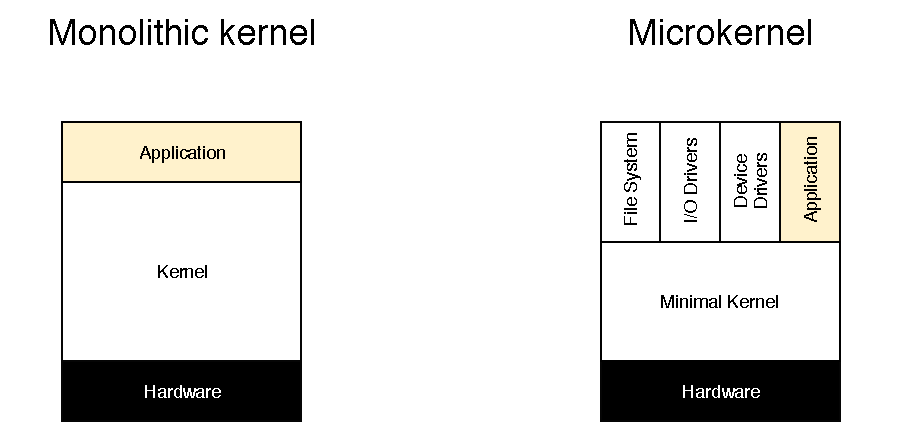
\includegraphics[scale=0.7]{assets/kernel_types.pdf}
    \caption{\label{fig:kernel-types}different kernel designs}
\end{figure}

% Others architectures
% Complete by mentioning other types?
Of course there are more architectures than what is listed above.
But in the context of this thesis, we considered that explaining in detail each one would not be relevant.
The two designs presented are the most common and provide a good preview of at what a kernel looks like.
Also, the following parts of this thesis will expand on this
    and we will see in practice what each RTOS uses from the theory.

\section{Scheduling}

The scheduler plays an important role in the design of a(n) (RT)OS.
The performances of an OS are deeply impacted by the scheduling algorithm it uses.
As we will see further in the thesis, it can also affect the energy consumption of the device.\\
%TODO reference for where

\subsection{Base concepts}

% What is a scheduler
A scheduler is a process designed to choose which task will run at a certain time in the system.
Different disciplines can be used, each one with multiple advantages and drawbacks.
Some commonly used are presented below in the Subsection 1.2.2.

% Preemptive vs non-preemptive (cooperative)
A scheduler is said to be \textit{preemptive} if tasks in the system can preempt each other.
When a higher-priority task wants to execute, the scheduler can interrupt a lower-priority task and run the higher-priority one.
In the other hand, a scheduler is said \textit{non-preemptive} or \textit{cooperative}
    if a task that has been allowed to start will execute until it is complete.

% online/offline
Another distinction we can make is to divide schedulers into \textit{online} and \textit{offline} schedulers.
% online
Online schedulers decide of the ordering of the different tasks during runtime based on various parameters (such as task priority for example).
A scheduler based on task priority is also called \textit{priority-based} scheduler.
% offline
On the contrary, offline schedulers (also known as \textit{table-driven} schedulers) perform their scheduling decisions at the start of the system.

The impact of these characteristics in the design of an RTOS will be explained later in this chapter.
%TODO reference

\subsection{Scheduling policies}

\subsubsection{First in, first out (FIFO)}
Also known as first come, first serve (FCFS), FIFO is one of the simpliest scheduling algorithm.
Processes are queued into a data structure in their order of arrival.
The first process to be enqueued is the first that will be executed.

\subsubsection{Round-robin}
The round-robin scheduling algorithm divides the time allocated to each process into fixed time slices.
If a process doesn not terminate when his allocated time slice is expired, the scheduler switches to another task.
If a task terminates within its time slice, the scheduler simply switches to the next task.

\subsubsection{Earliest deadline first (EDF)}
Earliest deadline first scheduling algorithm dynamically assigns a priority
    to each enqueued process (based on its deadline or an estimation of it) into a priority queue data structure.
The scheduler then executes the process the closest to its deadline at each scheduling event.

\subsubsection{Fixed-priority preemptive scheduling}
Priority for each task is pre-assigned by the operating system.
The scheduler arranges the tasks by order of priority.
Higher-priority tasks can interrupt lower-priority tasks.

%\subsection{Real-Time Scheduling}
%handbook chapter 2 12

\section{Memory management}

%https://www.memorymanagement.org/mmref/index.html#mmref-intro
%http://www.csc.twu.ca/rsbook/Ch12/Ch12.4.html
%https://www.gribblelab.org/CBootCamp/7_Memory_Stack_vs_Heap.html
%http://www.cs.virginia.edu/~son/cs414.f05/lec11.slides.pdf

In modern computer systems, memory management has evolved since early days techniques which were limited
    by early computer systems where each memory location was specified in the program.
This led to critical errors and/or unpredictability when an incorrect location was specified.

Nowadays, the memory management of (almost) every computer system follows the same principle:
the memory of a computer system can be divided into 2 distincts sections,
    the static memory (\textit{stack}) and the dynamic memory (\textit{heap}).

\subsection{Static memory management}
%stack
By the time a program begins to execute, there must be some specific blocks of memory reserved for its use.
This includes, for instance, the memory containing the program's own code.
Morever, every static variable must have a specific memory reserved.

The static memory allocation is predetermined by the compiler
    and will always be reserved for the program in the same manner at the beginning of every run.

This part of the memory operates as a \textit{stack} or last-in first-out (LIFO) queue.
The area of memory available for the use of the program will shrink and grow following the execution of the program,
which makes it very fast and efficient with no fragmentation.
%explain fragmentation?

\subsection{Dynamic memory management}
%heap
Sometimes, fixed memory size can be a problem.
Static memory does not allow allocation of memory beyond what is declared initially.
The \textit{heap} serves this purpose.
It is a large pool of memory which must be explicitly managed by the programmer.
It has no guarantee of efficient use of space, memory may become fragmented over time as blocks of memory are reallocated.

It may be tedious for the inexperienced programmer to manage the heap
    but it allows a more flexible and shareable pool of memory for an efficient programming.
To allocate memory on the heap, one must use \textit{malloc()} or \textit{calloc()} from the C code library stdlib.h (when available).
There are multiple algorithms to allocate memory when calling these functions.
The most common ones are presented below.

% conventional algorithms
\subsubsection{Sequential fit algorithm}
For this memory management algorithm, a single linkedvlist contains the unallocated blocks of memory.
When needed, they are allocated using different policies:
\begin{itemize}
    \item First fit: returns the first block large enough from the list.
    \item Next fit: similar to first fit but starts where the pointer was left off at the previous iteration.
    \item Best fit: research through the whole list and returns the smallest block large enough to meet the request.
    \item Worst fit: returns the largest block from the list.
\end{itemize}

\subsubsection{Buddy allocator algorithm}
This algorithm makes use of an array of linked lists.
Each list from the array owns blocks of a distinct size.
When requested, the buddy allocator algorithm finds the smallest but large enough block to meet the requirement from the array.
It then picks one of the block from this position in the array.

If the list is empty at the position where the best fitting block is located, it goes to the next position in the array
and splits a block from this list to fill the empty position.
The opposite can also be applied: two smaller blocks can be merged to obtain a bigger one.

\subsubsection{Indexed fit algorithm}
This algorithm makes use of an indexed data structure to implement the desired fit.
Some common data structures used for this algorithm are trees or hash tables.

\subsubsection{Bitmapped fit algorithm}
A bitmap representing the usage of the heap is created.
Each bit of the map corresponds to a part of the heap.
If a part is used, the bitmap is set to 1.
If not, it is set to 0.
Allocation is done by searching the bitmap for clear bits.

% unconventional algorithms?

%\subsection{Virtual Memory}
\section{Power management}

%to read
%https://dl.acm.org/citation.cfm?id=2333680
%https://dl.acm.org/citation.cfm?id=860179
%https://dl.acm.org/citation.cfm?id=860184
%https://ieeexplore.ieee.org/abstract/document/4054780
%http://www.es.mdh.se/pdf_publications/327.pdf
%https://www.sciencedirect.com/science/article/pii/S030626191630678X
%https://ieeexplore.ieee.org/abstract/document/5944309
%https://ieeexplore.ieee.org/abstract/document/8617010

%read
%https://www.sciencedirect.com/science/article/pii/S0167739X18329194


% \paragraph{}
% With the rise of cheap battery-powered embedded systems, the problem of energy efficiency becomes a non-negligeable stake.
% Each RTOS has its own way to manage its energy consumption.
% From a more general point of view, we can distinguish 2 ways to save energy in an embedded system.


% \subsection{Hardware energy management}

% At first, one could think that the hardware side of energy management is slightly out of context of the operating system means to save energy.
% The fact is that, even if we can distinguish 2 categories, the hardware means to save energy are very often tied to the upper layers of the whole system.

% \subsection{Software energy management}

The focus on energy management is something fairly recent in the field of information technology (IT).
With the rise of the Internet of Things (IoT), advancements have been made to allow operating systems to manage power consumption more efficiently.

Numerous communication stacks focused on IoT and low energy consumption have been developed in the last decade.
%TODO cite examples

Unfortunately lesser attention has been paid to the design of energy-efficient OS for resource-constrained devices.
Traditional hardware is limited in term of power management and the progress in this field required both software and hardware to evolve.
We will present below some of the advancements made and the technologies developed in recent years.


\subsection{Hardware power management}
In order to implement advanced techniques of power management, certain hardware features have been developed.
The purpose is to give more control from the software over the hardware.

\subsubsection{Clock gating}
% https://m.eet.com/media/1157354/fpmm%20-%20part%201.pdf
% https://en.wikipedia.org/wiki/Clock_gating
Clock gating is a technique consisting of turning off the clocks of unused peripherals in order to save energy.
Those peripherals enter what is called \textit{idle state} or \textit{sleep}.
The clocks are physically switched off from the circuit with the addition of a logical gate and do not consume energy until reactivation.

%power down mode? dynamic power
\subsubsection{CPU power down modes}
The recent advancements in CPU have introduced power-saving modes.
This feature stops the CPU clocks so that it is put to sleep unless
    a scheduling event or interrupt is triggered and wakes up the CPU, with the help of a real-time clock (RTC) for example.
% How the event can be scheduled if there is no clock to check the event ?

\subsubsection{Real-time clock wake up support}
% https://www.electronics-tutorials.ws/connectivity/real-time-clocks.html
When a CPU is in sleep mode, there is two possibilities to wake it up with an on-chip RTC or by an external event.
The on-chip RTC is a low-frequency clock (usually around 32kHz) that does not drain a lot of battery life.
RTC can include alarm functions: timers that when reached, trigger the RTC to wake up the processor.

\subsubsection{Supported CPU frequencies / dynamic frequency scaling}
In modern CPU, many options are available to switch between frequency ranges depending on the resources needed.
This feature can be used to minimize power consumption when  we do not need much computational power.

\subsubsection{Adaptive voltage scaling / dynamic voltage scaling}
%https://www.eetimes.com/document.asp?doc_id=1271842#
Similarly to the CPU frequency, voltage can be regulated based on the actual state of the chip.
The voltage is continuously monitored and adjusted during the runtime.


\subsection{Operating system power management}

\subsubsection{Peripherals state control}
Peripherals state control makes use of the clock-gating feature provided by the hardware.
Thanks to this feature, only the peripherals clocks required by the application at a certain point in time are active.
The other clocks are gated and do not consume energy.

\subsubsection{Sleep mode}
The idea is to allow the system to switch off certain components of the mi\-cro\-pro\-ces\-sor.

The sleep mode of a microprocessor takes advantage of multiple hardware features
    such as adaptative voltage scaling, CPU low-power modes and dynamic frequency scaling.
The RTC wake up support serves to wake up the CPU when in sleep mode and no other source is active.

\subsubsection{Tick suppression}
%https://www.embedded.com/electronics-blogs/industry-comment/4414162/1/FreeRTOS-s-tick-suppression-saves-power
Tick suppression defines the principle of providing tick-less support for the scheduler.

In a regular scheduler, a periodic timer (tick interrupt) is used to track time.
This tick interrupt wakes up the CPU to perform a scheduling cycle.
Such a mechanism, even if punctual, is frequent and then depletes power in a non-negligeable way by entering and exiting sleep mode frequently.

In a tick-less scheduler, the tick interrupt is disabled when the idle task is running.
Stopping the tick interrupt allows the CPU to remain in a deep power-saving state 
    until either an interrupt occurs or it is time for the kernel to switch task.

%schema tick vs tickless scheduler
\section{Programming model}
%definition
The programming model of an RTOS can be seen as "the way to program" an application using a specific RTOS.
Different "ways to program" or paradigms are predominant in the world of RTOS.
In this section, we will present the two main different paradigms used\cite{comparison_iot_constrained_devices}.


\subsection{Event-driven model}
In an event-driven programming model, a program generally consists of a main loop which listens for events.
Events can be generated by interrupts, sensors or user input.
When an event is detected, a callback function is triggered.

The developper has to manually maintain state across tasks which can be tedious.
Thus, the individual tasks do not have to maintain their own stack and they use a shared stack.
The memory footprint is then reduced since a single stack is used across the application.

\subsection{Multithreaded model}
The multithreaded model allows an application to run different tasks in their own thread context,
    and communicate between them using an IPC API.

Each thread has its own memory stack and does not require manual management by the programmer.
The stack is managed automatically by the thread scheduler.
The memory requirements of threaded application are often larger than their event-driven counterparts.
\section{Hardware support}

The embedded world is responsible for the majority of the world's microcontrollers.
The diversity of CPU keep increasing every year.
Working with this diversity of constrained devices makes the developer's work harder as he needs to adapt and learn to use specific librairies for each devices.
A source code on a particular device will not be easily reusable for another device.

With RTOS, developers can more easily make their code portable on many devices.

This section first describes the three constrained devices classes and how this is related to RTOS.
Then, it explains what an hardware abstraction layer (HAL) is and how a RTOS uses it in order to be compatible with the largest amount of devices.

\subsection{Constrained devices classes}

Constrained devices have been classified in 3 classes by the Internet Engineering Task Force (IETF) with the request for comments RFC7228 in May 2014.
%TODO cite rfc
IETF is a standards organization aiming at improving and maintaining the usability of the Internet.
Therefore they play a certain role in the evolution of IoT technologies.
We can argue that IETF is a competent authority over constraints devices since its domain of competence is the Internet.
Nonetheless, the boundary between constrained embedded devices and the Internet is permeable.
For the purpose of this thesis, the classification they made with RFC7228 is used.
RFCs are informational or experimental documents published by engineers and computer scientists.
Some of them become standards and some others \textit{de facto} standards.

The distinction between the three classes are made with the random-access memory (RAM) and read-only memory (ROM) capabilities of each device.
Table \ref{tab:constrained-devices-classes} resumes the different constrained devices classes.

\begin{table}[!h]
  \centering
  \begin{tabular}{|l|l|l|}
  \hline
   & Data size (e.g., RAM) & Code size (e.g., flash) \\ \hline
  Class 0 (C0) & \textless{}\textless{} 10 kB & \textless{}\textless{} 100 kB \\ %\hline
  Class 1 (C1) & $\sim$ 10 kB & $\sim$ 100 kB \\ %\hline
  Class 2 (C2) & $\sim$ 50 kB & $\sim$ 250 kB \\ \hline
  \end{tabular}
  \caption{classes of constrained devices}
  \label{tab:constrained-devices-classes}
\end{table}

\paragraph{Class 0.}
Those devices are the most constrained.
There are typically sensor nodes (or motes) in a sensor network.
There are so constrained that they cannot access Internet without the help of a larger devices.
The source code of a RTOS is often too heavy to fit in such devices.
Instead Class-0 devices are usually used bare metal.
In the embedded world, bare-metal programming is writing code that runs directly on the hardware without any abstraction such as an OS.

\paragraph{Class 1.}
Those devices are able to talk to each other but via constrained protocols.
The use of security protocols are often too heavy for that class.
%RTOS mainly target this kind of devices.
RTOS generally require at least a few kB for the strict minimal functionalities to run.
Therefore, they are not practical for class 0 devices (even if they could technically run) and mainly target class 1 or more powerful devices.


\paragraph{Class 2.}
Those devices are the less constrained and can use the same stacks of protocols used in personal computers and servers.
General-purpose OS can be used for this kind of devices but the class-2 devices can benefit from lightweight and energy-efficient protocols.

\subsection{Hardware abstraction layer}

Due to the variety of CPU, vendors provide a set of libraries used to develop applications on their architectures.
This set of libraries and tools are called the hardware abstraction layer.

\paragraph{Definition of HAL}
% TODO
% Repetition of 'hardware'
A hardware abstraction layer defines a set of routines, protocols and tools to access underlying hardware.
It provides abstract and high-level functions to interact with the hardware.
The hardware, drivers and board supports are considered as black-boxes.

\paragraph{RTOS and HAL}
The HAL is strongly dependent on the architecture of the CPU.
In order for the RTOS to support multiple boards and architectures, it has to implement and use the different HAL provided by the vendors.

\begin{figure}[!h]
  \centering
  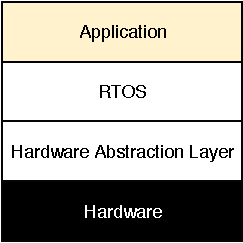
\includegraphics[scale=1]{assets/hal-layers.pdf}
  \caption{\label{fig:hal-layer}layers around the hardware abstraction layer}
\end{figure}

Figure \ref{fig:hal-layer} shows that the application and RTOS layers are placed above the HAL, itself just above the device layer.
The application layer talks to the RTOS and the RTOS layer talks to the corresponding HAL depending on the device used.

%TODO rework this part
\paragraph{Pro and cons}
Developers can switch hardware and perform cross-platform testing more easily.
But there is some limitation: the HAL is tied to the hardware and change heavily with it.
Also, there is some limitation using an hardware abstraction layer.
Not all the functionalities from the hardware are available.


